The same quantum mechanical system can have different states that are described by wavefunctions of different complexity.
An example might be the behavior of a system as it approaches a specific temperature.
This could be the \emph{boiling point} of a fluid, at which the liquid turns into steam and starts behaving completely differently.
It could also be the approach to \emph{absolute zero}, that is commonly known to be responsible to induce unique behavior in quantum objects.
Depending on the nature of the system, the approach to such a point could make the wavefunction simpler or more difficult to parameterize.

Temperature is not the only parameter that could induce a transition, which is generally known as a \emph{phase transition}.
In our case the \emph{strength of the transverse electromagnetic field} can also cause such a phase transition.

The location of the transition is dictated by the ratio of the Ising parameters $J$ and $h$, $\lambda = \frac{h}{J}$, as well as the shape and dimensionality of the lattice.
The experiments in the preceding sections all used a $\lambda = \frac{h=-0.7}{J=-1} = 0.7$.
In the book \emph{Quantum Ising Phases and Transitions in Transverse Ising Models} \cite{isingBook}, the transverse field Ising phase transition is said to occur around $\lambda = $ \SIrange[]{2}{4}{} for 2D latices of square nature.

\begin{figure}[htbp]
    \centering
    \makebox[\textwidth][c]{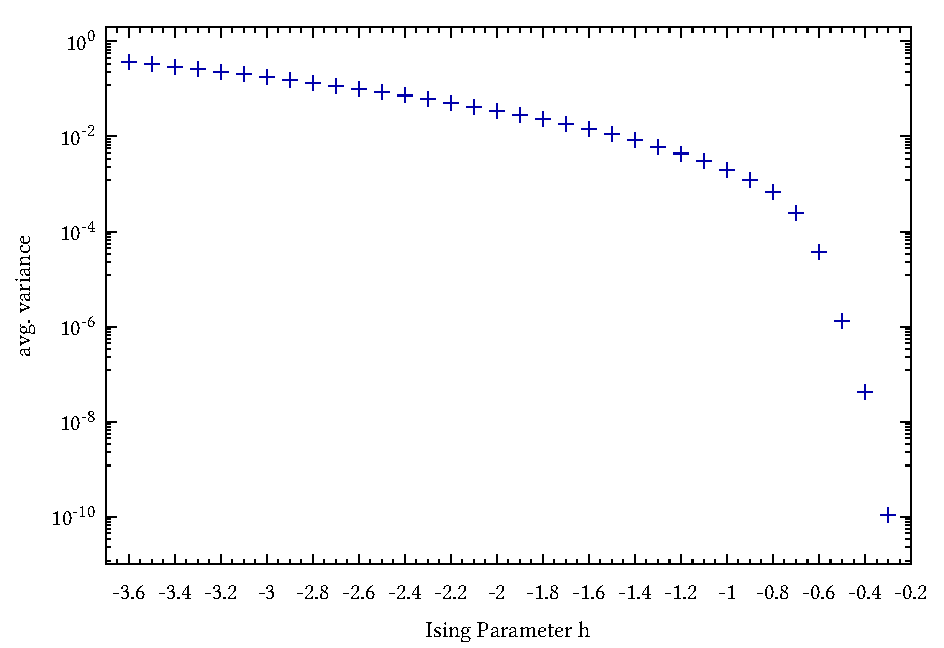
\includegraphics[width=1\textwidth]{./experiments/ground-state-search/differences-phase-diagram/phase-transition/phase-transition.pdf}}
    \caption{
        A ground state search was performed with a CNN as a NQS for different values of the Ising parameter $h$.
        The recorded values are an average of the energy variance in the logarithmic scale for about 500 steps after the CNN had converged.
        The lattice is of the trigonal\_square type, with periodic boundary conditions and a size of 4 (64 lattice sites).
        The Ising $J$ parameter as always set to -1.
    }
    \label{fig:phase-transition}
\end{figure}

Experiments with a CNN on a periodic 2D-trigonal\_square lattice around the region of $J = -1$, $h = $ \SIrange[]{-0.3}{-3.6}{} show significant differences for the minimal achievable variance (\autoref{fig:phase-transition}). 
For some $\lambda$, the smallest variance the CNN achieved was larger by several orders of magnitude compared to the experiments in the past sections.
Bringing the $h$ parameter closer to zero, made the minimum variance drop quickly ($\approx 0.02$ for $h = -1.8$ down to falling to $< \SI[]{10e-3}[]{}$ for $h \geq -0.8$).
From $h = $ \SIrange[]{-2.5}{-3.6}{} the minimum variance rises approximately linear on the logarithmic scale. 
This suggests representing the wavefunction gets exponentially harder for the CNN as $\lambda$ grows.

\begin{figure}[htbp]
    \centering
    \makebox[\textwidth][c]{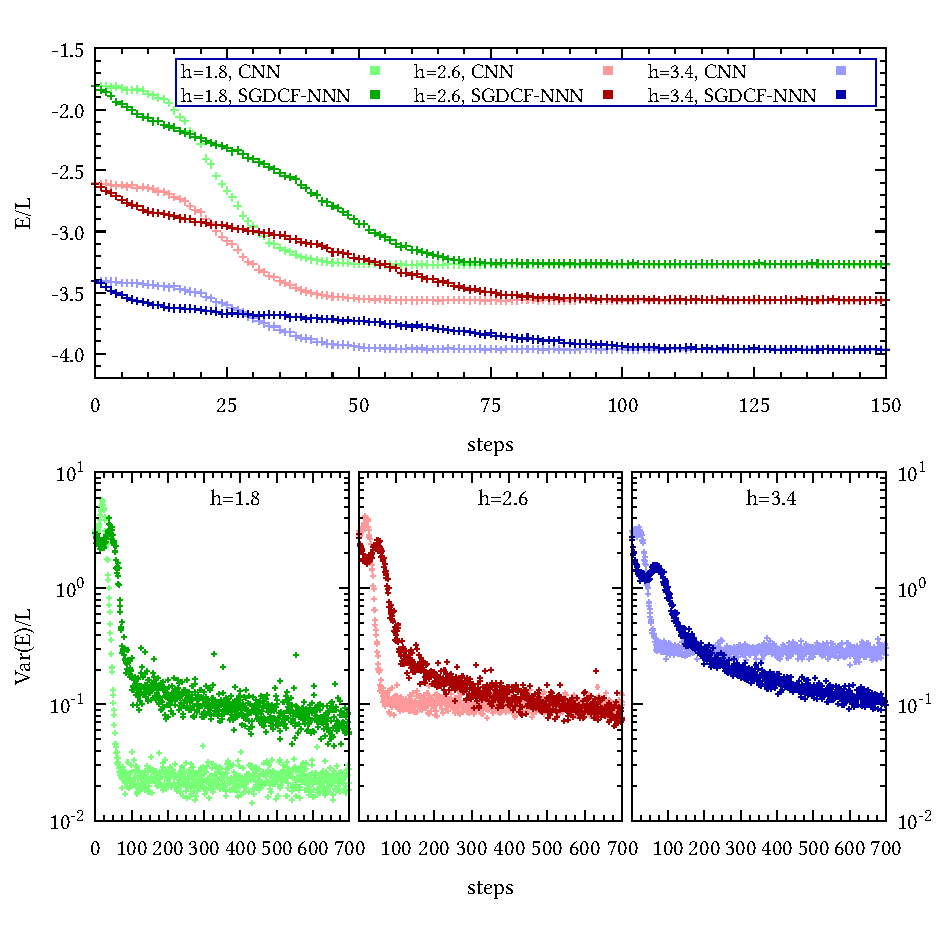
\includegraphics[width=1.1\textwidth]{./experiments/ground-state-search/differences-phase-diagram/performance-across-phase/performance-across-phase.pdf}}
    \caption{Detailed depiction of a selection of runs from the experiment shown in \autoref{fig:phase-transition}.
        The CNN and lattice configuration are the same in both cases.
        Additionally the same problem was solved with a SGDCF-NNN as the NQS.
        The depthwise graph conformer was configured with a depth of 2, an embed dimension of 9 and a mlp-ratio of 2.
        The Ising $h$ parameter and therefore the different values of $\lambda$ are encoded in the curve's color. 
        The CNN is depicted in the light shade, the SGDCF-NNN in the dark.
    }
    \label{fig:performance-across-phase}
\end{figure}

The reason for operating close to the phase transition region is exactly this increasing complexity of the wavefunction.
Previous sections suggested, that the metaformer architecture might be too \glqq complex\grqq{} to represent the basic wavefunctions around $\lambda = 0.7$. 
This might be the reason, why the extremely simple CNN is outperforming the sophisticated metaformer in these examples.

\autoref{fig:performance-across-phase} validates this theory.
For three different values of $\lambda$, the CNN and a SGDCF-NNN metaformer are compared. 
The conformer was set up to have a slightly smaller footprint than the CNN (CNN: 1024 parameters, SGDCF-NNN: 972 parameters).
For the smallest value of $\lambda = 1.8$, the two networks behave the same way as in \autoref{sec:experiments-comparisontoestablished}. 

But by raising the value of $\lambda$ to \SI[]{2.6}[]{}, the conformer may finally make use of its more specialized design.
The red colored curves show the two models successfully rivaling each other in terms of the minimum variance.
The conformer even being slightly ahead.
This can be attributed to the conformer keeping its level of performance constant, even though the CNN performs noticeably worse on this wavefunction.

For even larger values of $\lambda$ - supposedly close to the \emph{critical point} of the phase transition - the CNN's accuracy collapses. 
For $\lambda=$ \SI[]{3.4}[]{} (blue curves), the minimum variance of the CNN is approximately one order of magnitude worse than for $\lambda=$ \SI[]{1.8}[]{}.
As the conformer is still performing without a noticeable dropoff in accuracy, it is at this stage able to surpass the CNN and parametrize the wavefunction in a better way than its adversary.

Finally it is important to point out, that in all cases the conformer variance was still dropping at the end of the calculation, while the CNN's variance had clearly already converged.
And even though the conformer had a smaller number of trainable parameters, it was able to outperform the established CNN for large enough $\lambda$ due to its strong consistency across the phase domain.

None of the architectures is perfect, as both showed unstable calculations in the regions of $\lambda < 0$. 
As e.g. all of the tested models quickly crashed due to \emph{NaN} errors for $\lambda = -3.6$, it is safe to say that not all problems can be solved by the metaformer framework.
Though the experiments show that they provide a great deal of flexibility and resiliency against several difficulties posed by the computational problems.

Further exploration of metaformer concept inside the phase transition regions promises to provide an excellent opportunity for further research in this domain.
